\chapter{Project Premise and OPNET Model Design} 

This chapter presents the premise and details of a specialized network design used to analyze message ferrying in section \ref{sec:premise}.
A general overview of the OPNET model which was created is then presented in section \ref{sec:model_design}.
Please refer to the appendix for specific details.
Finally, the results of an initial simulation used to validate the node models is presented in \ref{sec:validation}.

\section{Premise}
\label{sec:premise}

This section outlines the requirements for any application which uses message ferrying.
Details of a specialized \lq{}state monitoring\rq{} network are then discussed.

\subsection{Application Characteristics and Requirements}
\label{sec:premise_appchar}

Any application making use of message ferrying must have the following characteristics:

\begin{description}
\item[Delay Tolerance: ]
Since data is transported by a physical device, significant delays of minutes to hours must be expected.
\item[Loss Tolerance: ]
Given that ferries have limited memory, loss of data must be expected.
\item[Small and Independent Messages: ]
Following from the limited memory capacity of ferries and the high probability of data loss, a reliable method for segmentation and reassembly of messages should not be expected. 
Applications should limit the size of messages such that the can be transmitted in their entirety using one protocol data unit.
\end{description}

Given these criteria, a message ferrying network is unsuitable for many typical networking applications including web browsing, real-time voice or text communication and file transfer.
As such, a very specialized 'state monitoring' network designed for non-critical monitoring of remote sensors is considered.

\subsection{State Monitoring Network}

The general premise for this project consists of a network containing numerous, uniquely identifiable source nodes. 
Each source node has a limited number of properties, in the form of key/value pairs, specifying a property name (the key) and its current value.
Properties may change overtime and each change defines a new state for the source node.
A temperature sensor for example, might support a 'temperature' property, the value of which is the current temperature updated every hour.
Properties do not have to contain a single value and each may be as large as the payload limit of network packets. 

The network and message ferrying algorithm is designed to synchronize a central repository with the current state of every source node.
Only the most recent state (or most recent value) for each property is important, not the history of how that property has changed.
This limits the number of packets which can exist in the network as only the most recent update must be reported.
The message ferries collect data from source nodes when they are in range and transport it to the central repository.
The central repository is assumed to be a server connected to the Internet.
Ferries pass updates they have collected from source nodes to special gateway nodes.
These gateway nodes are then responsible for using a reliable delivery mechanism over a standard IP network to update the central repository.
This last stage is not considered for the implementation presented here.
Once messages have been delivered to gateway nodes, they are assumed to have been delivered.

%--------------------------------------------------------------------------------------------------------
% 		Design
%--------------------------------------------------------------------------------------------------------
\section{OPNET Model Design}
\label{sec:model_design}

Due to the lack of support in OPNET for message ferrying, all node and process models were creates specifically for this project. 
An overview of the basic network elements, including node and packets types, is presented in \ref{sec:net_element}.
A description of the networking algorithm is then presented in section \ref{sec:algorithm}.
Please refer to the appendix for specific implementation details.

\subsection{Network Elements}
\label{sec:net_element}

\subsubsection{Network Nodes}

The network is comprised of three types of network nodes:

\begin{description}

\item[Source Node: ] 
Static (non-mobile) nodes in the network which have a set of properties (key/value pairs).
After a property of a source node changes, known as a state change, it attempt to notify the central repository via gateway nodes by transferring update packets to any message ferries which are in range.
It is important to note that source updates may be delivered to any gateway.
A source node could be, for example, a remote temperature sensor.
\item[Message Ferry: ] 
Mobile nodes which collects updates from source nodes when they are in range.
Message ferries store updates from source nodes within a buffer. 
When in range, these update packets are forwarded to gateway nodes.
A source node could be, for example, a specially equipt cell phone or a small computer attached to a vehicle. 
\item[Gateway: ]
Gateway nodes download update packets from message ferries and mark them as received.
\end{description}

Source nodes have properties (prop1, prop2, etc) which generate update messages. 
These messages get carried to \emph{any} gateway node by message ferries. 
The OPNET node model for a source node node may be seen in \ref{fig:source}

\begin{figure}[h]
    \centering
    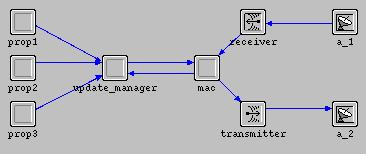
\includegraphics[width=.7\textwidth]{images/source.jpg}
    \caption{Source Node Model}
    \label{fig:source}
\end{figure}

The OPNET node model for a message ferry is shown in figure \ref{fig:Ferry}.
The ferry is a mobile node which collects updates from source nodes when they are in range. 
These updates are then stored in memory (the storage process in figure \ref{fig:Ferry}). 
The storage process compares the updates, uniquely identified by source ID and property key, and keeps the most recent according to the key update number (see below).

\begin{figure}[h]
    \centering
    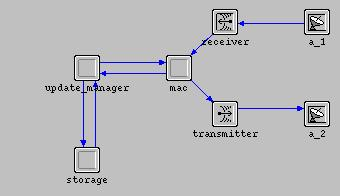
\includegraphics[width=.7\textwidth]{images/ferry.jpg}
    \caption{Ferry Node Model}
    \label{fig:Ferry}
\end{figure}

The OPNET model for a gateway node is shown in figure \ref{fig:Gateway}. 
The gateway process model seen in the figure is responsible for tracking what updates have been received.
It makes use of global variables so updates may be received by any gateway.

\begin{figure}[h]
    \centering
    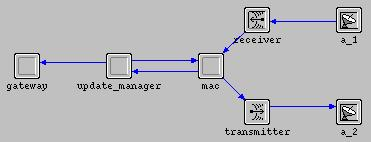
\includegraphics[width=.7\textwidth]{images/gateway.jpg}
    \caption{Gateway Node Model}
    \label{fig:Gateway}
\end{figure}

\subsubsection{Properties and Property Process}

Each source node supports three properties as can be seen in figure \ref {fig:source}.
Furthermore, each property has three main pieces of data as described below. 
Updates generated by the property contain these three pieces of information.
For the purposes of this project, the value of the property is inconsequential and not considered.

\begin{description}
\item[Source ID: ] A unique identifier of the source node a property is associated with
\item[Key: ] Or property key is a unique for each property within a source node
\item[Key Update Number: ] A counter which is incremented each time the property value changes. 
Only the most recent value of a property, as defined by its key update number, is of importance.
\end{description}

\subsubsection{Packets}

Two types of packets are used within the OPNET model.

\begin{description}
\item[Update Packet: ]
Update packets are generated by the property processes of source nodes when their value changes.
They are transmitted to message ferries which in turn transport them to the gateway.
\item[Beacon Packet: ] 
Beacon packets are used to detect when nodes are in range and are able to communicate.
Beacon packets are generated periodically be ferry and gateway nodes and trigger transmission of stored update messages by receiving nodes.
\end{description}

%--------------------------------------------------------------------------------------------------------
% 		Algorithm
%--------------------------------------------------------------------------------------------------------
\subsection{Algorithm and Behaviour}
\label{sec:algorithm}

A brief overview of the algorithm implemented in each node is presented in this section.
Pseudo code is presented here; refer to the appendix for the actual implementation.

\subsubsection{Ferry Node Algorithm}

Ferry nodes behave in the following way. Note that ferry nodes are mobile.

\begin{enumerate}
\item Periodically send beacons to notify other nodes that there is a ferry in range.
These beacons trigger source nodes and other ferries to transmit stored updates.
\item When updates are received, store them.
Updates are discard based on the following conditions.
	\begin{enumerate}
	\item If two updates (one received and one in memory) with the same source id and key are detected, discard the updated with the smallest key update number.
	\item If the memory limit has been reached, discard the oldest update (regardless of source id and key).
	\end{enumerate}
\item When a beacon is received, transmit all updates in memory.
\item Repeat
\end{enumerate}

\subsubsection{Source Node Algorithm}

Source nodes behave in the following way

\begin{enumerate}
\item Wait for a beacon.
\item Based on the current state, defined by the key update number for each property, transmit updates.
\item Repeat
\end{enumerate}

\subsubsection{Gateway Algorithm}

Gateway nodes behave in the following way:

\begin{enumerate}
\item Periodically send beacons to notify other nodes that of the gateways existence.
\item Wait for updates to be received
\item If an update received for a given source id and key has a greater key update number than the last update received for that source id and key, record an update.
If the key update number is equal to or less than the last update, discard the update.
\end{enumerate}

\subsection{Assumptions}

In order to simplify the simulation and focus on the message ferrying algorithm, a number of assumptions were made regarding data transmission and wireless communication.

\begin{itemize}
\item Communication range of 60 meters.
When nodes are closer than 60 meters they can communicate and when they are further apart than 60 meters, they cannot.

\item No propagation and transmission delay.
This assumption was made to ensure ferries receive all updates when moving past source nodes.

\item No unintentional loss, the node link is assumed to be reliable. 
It is assumed that there is no loss caused by radio interference. 
This assumption was made to eliminate the need for an acknowledgment and retransmission mechanism.

\end{itemize}

These assumptions are considered valid as there are are number of technologies, implemented at a lower network layer, which provides reliable data transfer services.

%--------------------------------------------------------------------------------------------------------
% 		Validation
%--------------------------------------------------------------------------------------------------------

%This section needs to be changed a lot
%Lets break it down into 'validation' and put that in the previous section
%
%I am adding another section which talks about the 'main' simulation

\section{Validation} %TODO: no longer a chapter

%small intro
In this section, we will discuss the simulation to validate our design and implementation. 
A scenario is created to validate that the updates from source nodes are delivered successfully when in range to the ferry node and the update packets are handled properly by the ferry node as designed.   
Further detail will be explained in the following subsequent section \ref{sec:scenario1}. %might remove this line


%When simulating each scenario, the following metrics will be measured:
%\begin{enumerate}
%	\item Time to update state in central repository (delay)
%	\item Variation in time to update state (delay jitter)
%	\item Number of state updates lost. Roughly corresponds to packet loss.
%	\item Memory utilization and packet dropping threshold within ferries.
%\end{enumerate}

%_________________________________________________________________
%________________________SCENARIO 1_______________________________
\subsection{Scenario Topology  and Details}
\label{sec:scenario1}


In Figure \ref{fig:scenario1}, it shows the topology to test if the gateway receives the update packets sent by the source nodes and if the ferry is picking up these update packets from source nodes when it moves past them.
There is one gateway node, one ferry node, and seven source nodes. 
The size of this topology is 0.75km x 0.75km with source nodes placed evenly apart by 0.375km. 
The gateway node is on the top left corner, and the ferry is in motion indicated next to a red arrow.
The speed of the ferry is a constant 60kph, as it moves clockwise two times along the rectangular path that is highlighted in white.  The simulated time is six minutes.

%picture of the rectangular path
\begin{figure}[ht]
    \centering
    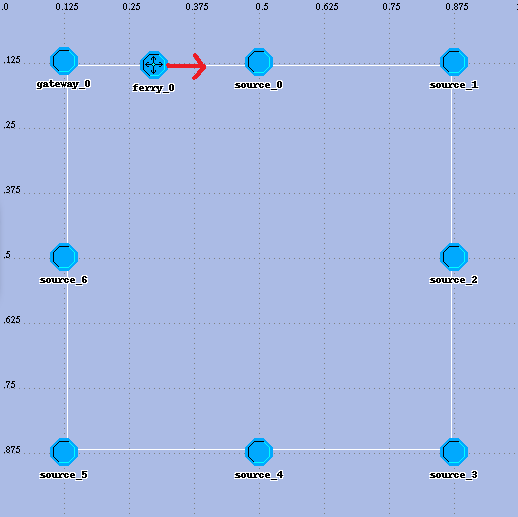
\includegraphics[width=.5\textwidth]{images/scenario1-top1r}
    \caption{Validation scenario topology}
    \label{fig:scenario1}
\end{figure}

\subsection{Validation Simulation Results}
\label{sec:results-validate}


After setting up OPNET to capture the desired statistics, the design and implementation are simulated.  The results are collected and shown in Figure \ref{fig:result1-a}.  From it, we can see that the ferry is picking up three update packets each time it passes by a source node.  This validates that ......

%result1-a   ferry receives update packets
\begin{figure}[ht]
    \centering
    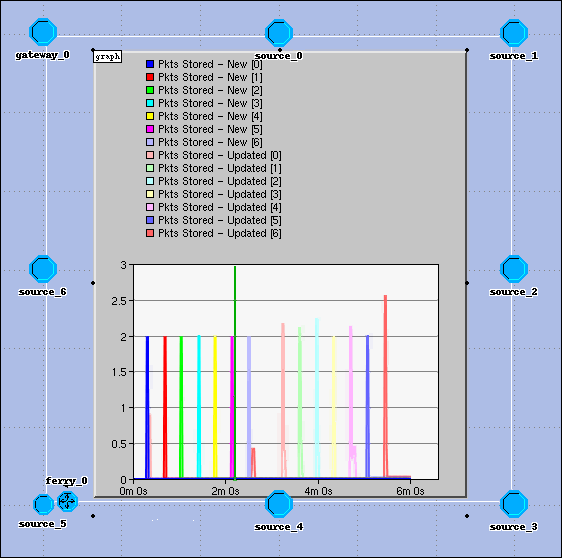
\includegraphics[width=.5\textwidth]{images/scenario1-result-received}
    \caption{Update packets received by the fery node}
    \label{fig:result1-a}
\end{figure}

The second part of the results is to see the if the gateway receives the update packets collected by the ferry node.  From Figure \ref{fig:result1-b}, there are two spikes in the graph which corresponds to the task of dumping the packets to the gateway node.  
The ferry node goes around two times for this simulation and that is why we see we two spikes.  
Each source node sends three update packets to the ferry node as it passes.  
Since there are seven source nodes, this accounts for the 20 packets received by the gateway node, which can be seen in Figure \ref{fig:result1-b}.


%result1-b   ferry delivers update packets to gateway
\begin{figure}[ht]
    \centering
    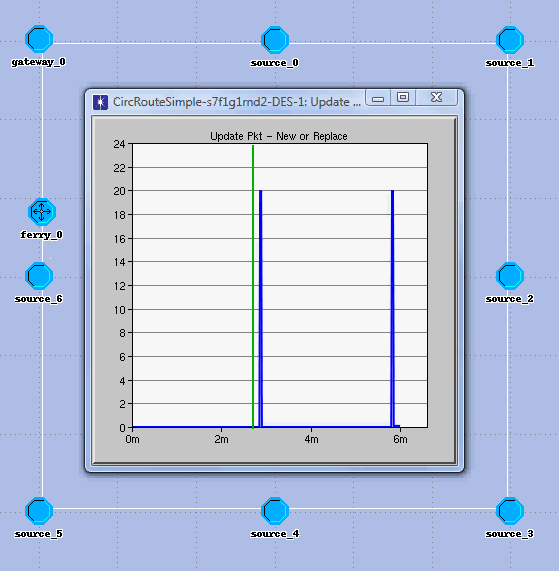
\includegraphics[width=.5\textwidth]{images/scenario1-result-gateway}
    \caption{Gateway receives the packet as the ferry node passes by its range of transmission}
    \label{fig:result1-b}
\end{figure}

